%
%       titel.tex - Titelblatt
%
% --- ! Anpassungen sind nur GANZ UNTEN erforderlich !  ---
%
% ---------------------------------------------------------
%       Diese Datei ist Teil der LaTeX-Vorlage fr
%             Studien-und Diplomarbeiten am
%    Institut fr Mechanik und Meerestechnik, TUHH
%
% (c) Institut fr Mechanik und Meerestechnik
%     Technische Universit� Hamburg-Harburg
%     2006
%
% Weitere Informationen finden Sie in  diplomarbeit.tex .
% ---------------------------------------------------------
%
%

% ------------ Definition der Befehle ---------------
%       (hier sind keine Aenderungen noetig !)

% \deckblatt{Rand}{Seitenbreite}{Kopftext}{Fensterbreite}{Fensterhoehe}{Fenstertext}{Untertext}{Fusstext}
%
% Rand:          zusaetzlicher rechter Rand zur Ausrichtung der Seite auf das Sichtfenster
% Seitenbreite:  Seitenbreite
% Kopftext:      Text ueber dem Sichtfenster
% Fensterbreite: Breite des Sichtfensters
% Fensterhoehe:  Hoehe des Sichfensters
% Fenstertext:   Text im Sichtfenster
% Untertext:     Text unter dem Sichtfenster
% Fusstext:      Text nach \vfill

\newcommand{\deckblatt}[8]{
  \begin{titlepage}
  \vspace*{-20mm}
  \hspace{#1}               % Ausrichtung zum Sichtfenster, auch unten
  \begin{minipage}[t]{#2}       % Minipage Titelseite
    \begin{center}
    \begin{minipage}[t][64mm][t]{#2}    % Minipage Kopf
      \begin{center}
      #3
      \end{center}
    \end{minipage} \\           % Minipage Kopf
    \vspace{10mm}
    \begin{minipage}[t][#5][c]{#4}  % Minipage Sichtfenster
      \begin{center}
      #6
      \end{center}
    \end{minipage} \\           % Minipage Sichtfenster
    \vspace{26mm}
    #7
    \end{center}
  \end{minipage} \\         % Minipage Titelseite
  \vfill
  \hspace{#1}               % Ausrichtung der Titelseite zum Sichtfenster
  \begin{minipage}[t]{#2}      % Minipage Datum
    \begin{flushright}
		#8
	\end{flushright}
  \end{minipage}            % Minipage Datum
  \end{titlepage}
}

% \titelseite{Fenstertext}{Untertext}{Fusstext}

\newcommand{\titelseite}[3]{%
  \deckblatt{1mm}{175mm}{
    \vspace*{15mm}    
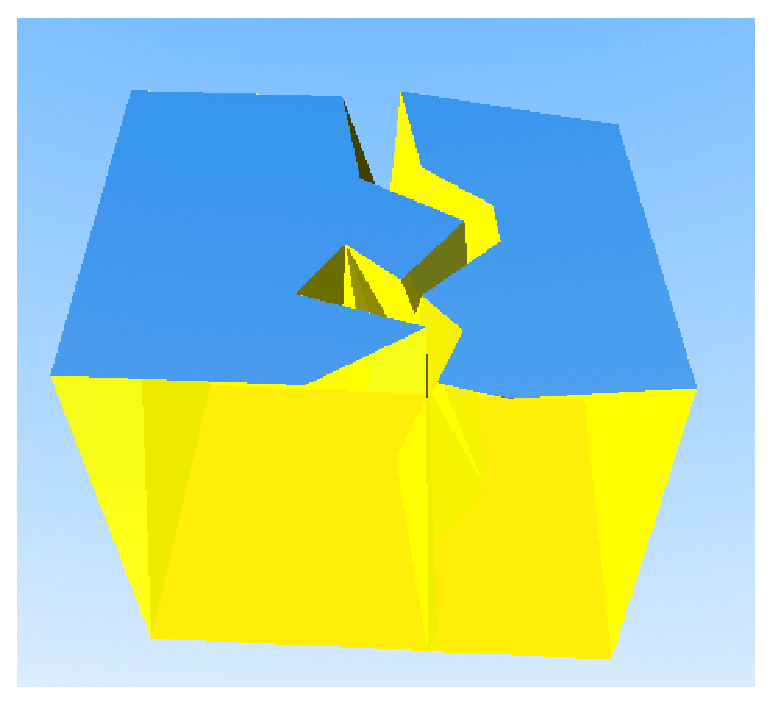
\includegraphics[width=65mm]{/home/java/Documents/Tex/Tex/vrml.eps}
  }{105mm}{65mm}{#1}{#2}{#3}
}

% ------------------ ! Text hier anpassen ! ------------------------

% Schema:  \titelseite{Fenstertext}{Untertext}{Fusstext}
% Fenstertext:   Text im Sichtfenster
% Untertext:     Text unter dem Sichtfenster
% Fusstext:      Text nach \vfill

\titelseite{
  % Fenstertext
  {\large \bf Diplomarbeit} \\  [7mm]
  {\LARGE \bf Berechnung beweglicher Objekte aus Beobachtungen}\\[7mm]
  {vorgelegt von} \\[7mm]
  {\large Andreas Ruloffs}\\
  {\large 6~65~11~19}
}{
  % Untertext
\begin{flushright}
  Betreuer: \\[5mm]
  Prof. Dr.Ralf Hartmut G"uting \\[12mm]
   \begin{floatingfigure}[r]{20mm}
      
\includegraphics[width=20mm]{/home/java/Documents/Tex/Tex/feu_logo2.eps}
   \end{floatingfigure}
\textbf{FernUniversit"at}\\
Gesamthochschule Hagen\\
Fachbereich Informatik\\
Lehrgebiet Praktische Informatik IV
\end{flushright}
}{
  % Fusstext
 Gelsenkirchen, Mai 2008}